\chapter{Social Choice}
\label{c:social-choice}

So far, we've been focused on the question of individual choice.  How should a single individual choose from among several different options?  In this chapter, we will go up in scale, and ask the same question about a group.  How should a group  decide given the preferences of its members?

A group could be anything: a country, a company, an organization, even a small group of friends.  The basic question is the same: what is the best way to put together a collection of preferences into a single ``group preference'' that appropriately reflects the preferences of the members?

Also unlike in the previous chapters, this one will have more disappointing conclusions.  Whereas the last several chapters have focused on proving that something was possible, these chapters will highlight how difficult group decision-making is.  

In some sense, this is a relief.  Anyone who's lived through the last few decades knows that democracy is hard.  This chapter can be seen as giving a kind of mathematical explanation.

\section{A little formalism and a problem}

As we have with basically every chapter, we will start with a set of options $X$.  We will assumed that $X$ is finite, but could be very large. We're assuming that $X$ represents whatever the group is hoping to decide. {\it Critically,} we will assume that there are at least three members in $X$, that the group has more than two options available to them.  This is a very critical assumption, many of the results we state will not be true if there are only two options.

If we are thinking of electing a leader, then $X$ will have all the candidates.  If a group of friends is deciding where to go for dinner, then $X$ is a set of restaurants.  As before, $X$ should make up a set of mutually incompatible things, we are choosing one and only one.

We will assume, also, that there is a set $N$ of people.  These are all the relevant people in the group: those whose opinions matter for the purposes of making a decision. If we're thinking about an election this might be every eligible voter or at least everyone who actually votes. For a group of friends, this should be every friend.  

Some care must be given to this, since it's important that anyone who {\it might} have a say, should be included in $N$.  If we leave some people out, then the model is missing something.

We will assume that each person in $i \in N$ has a (potentially different) preference relation $\succsim_i$ over $X$.  We will assume that each $\succsim_i$ is transitive and complete.  But we will not go any further than this. We won't use either von Neumann\breakslash Morgenstern or Anscombe\breakslash Aumann axioms.  For the moment, just go with me on this. I will come back to it in the next section.

We will use the set $R$ to collect all possible complete and transitive preference relations over $X$.  The idea is that the set $R$ contains all possible opinions that someone might have.  Each individual will then be identified with one of those relations.  A relation might occur twice (or more) in a group, since two people might have the same opinion.  

A ``community profile'' will then be a vector of preference relations with $N$ entries.  We can think of a group of people as defined by $\langle \succsim_1, \succsim_2, \dots, \succsim_n\rangle$.  This tells us what person 1 wants, what person 2 wants, etc.

Before we go any further, we should take a second and talk about a particular community profile that is a problem.  This was discovered by a relatively early champion for the mathematical way of looking at democracy: Marie Jean Antoine Nicolas de Caritat, Marquis of Condorcet.  Yes, that's actually his name.  We will just call him Condorcet.

Consider a group of friends trying to decide where to have dinner.  Let $X = \{$ Bennie's BBQ ($b$), Connie's Kitchen ($c$), Donnie's Dinner ($d$)$\}$  Condorcet discovered this profile, called the Condorcet cycle or Condorcet ``paradox:''
\begin{itemize}
    \item Mandy: $b \succ c \succ d$
    \item Evan: $c \succ d \succ b$
    \item Stephanie: $d \succ b \succ c$
\end{itemize}

First, let's think about what would happen if everyone voted on where to go by choosing their favorite and voting for it.  Now there would be three-way tie for where to go: each restaurant would get one vote.  It wouldn't get any better if we had people submit their ranked list because each restaurant would get 1 first-place, 1 second-place, and 1 third-place vote. So that doesn't help either.

Mandy might propose that they decide this way: ``let's first decide on $c$ vs. $d$. Then the winner will be put up against $b$.''  Let's assume they did this, and everyone voted in every round according to their preference.

This would create a kind of bracket like this like in figure~\ref{f:cc-first-vote}.  In this vote, $c$ would beat $d$ by a vote of 2:1.  (Mandy and Evan prefer $c$ to $d$.) Then when $c$ is put up against $b$, $b$ would win again by 2:1. (Mandy and Stephanie both prefer $b$ to $c$.)

\begin{figure}
\centering
\begin{tikzpicture}%
[ every text node part/.style={draw, align = left, inner sep = 0pt} ]

% Setup for horizontal tree
    % Grow tree to right with nodes placed clockwise(')
    \tikzset{grow'=left}
    % Use edges with 90° bends instead of default straight
    \tikzset{edge from parent/.style = { draw,
             edge from parent path = { (\tikzparentnode.west) 
                                        -- +(-8pt, 0)
                                        |- (\tikzchildnode.east) }}}
    % Increase horizontal spacing (adjust if length of name is long)
    \tikzset{level distance = 7em}
    % Adjust the alignment of the nodes
    \tikzset{every tree node/.style = {draw, anchor = base west}}

\Tree[ .{$b$ (winner)} {$b$ (2 votes)} [ .{$c$ (1 vote)} {$c$ (2 votes)} {$d$ (1 vote)} ] ]
\end{tikzpicture}
\label{f:cc-first-vote}
\caption{One way of running an election for the Condorcet cycle}
\end{figure}

But that's just way of running the election.  What if we switched it around? 

\begin{figure}
\centering
\begin{tikzpicture}%
[ every text node part/.style={draw, align = left, inner sep = 0pt} ]

% Setup for horizontal tree
    % Grow tree to right with nodes placed clockwise(')
    \tikzset{grow'=left}
    % Use edges with 90° bends instead of default straight
    \tikzset{edge from parent/.style = { draw,
             edge from parent path = { (\tikzparentnode.west) 
                                        -- +(-8pt, 0)
                                        |- (\tikzchildnode.east) }}}
    % Increase horizontal spacing (adjust if length of name is long)
    \tikzset{level distance = 7em}
    % Adjust the alignment of the nodes
    \tikzset{every tree node/.style = {draw, anchor = base west}}

\Tree[ .{$c$ (winner)} {$c$ (2 votes)} [ .{$d$ (1 vote)} {$b$ (1 vote)} {$d$ (2 votes)} ] ]
\end{tikzpicture}
\label{f:cc-second-vote}
\caption{A second way of running an election for the Condorcet cycle}
\end{figure}

And, of course, there is a third way

\begin{figure}
\centering
\begin{tikzpicture}%
[ every text node part/.style={draw, align = left, inner sep = 0pt} ]

% Setup for horizontal tree
    % Grow tree to right with nodes placed clockwise(')
    \tikzset{grow'=left}
    % Use edges with 90° bends instead of default straight
    \tikzset{edge from parent/.style = { draw,
             edge from parent path = { (\tikzparentnode.west) 
                                        -- +(-8pt, 0)
                                        |- (\tikzchildnode.east) }}}
    % Increase horizontal spacing (adjust if length of name is long)
    \tikzset{level distance = 7em}
    % Adjust the alignment of the nodes
    \tikzset{every tree node/.style = {draw, anchor = base west}}

\Tree[ .{$d$ (winner)} {$d$ (2 votes)} [ .{$b$ (1 vote)} {$b$ (2 votes)} {$c$ (1 vote)} ] ]
\end{tikzpicture}
\label{f:cc-third-vote}
\caption{A third way of running an election for the Condorcet cycle}
\end{figure}

So now instead of debating which restaurant to go to, each friend will debate the proper way to structure the election. We could have them vote on that, but that's no help because we'll just generate another Condorcet cycle.

The basic problem is this: for any restaurant you choose, the majority will prefer a particular alternative to the one that is chosen.  This happens regardless of which one is chosen, so as a result no particular solution appears ``best.''

\section{What about utilities?}

After we spent all this effort trying to figure out utilities, it might seem natural to use them in this context.  While the Condorcet cycle is perplexing, perhaps we could resolve the problem by asking people not just what is their preference, but by how much they prefer it.  In fact, we do this all the time\dots but maybe we shouldn't?

The first thing to note is that this can't eliminate the Condorcet cycle entirely. We could also specify that everyone's strength of preference is exactly the same and be back where we started.

But, actually there is a deeper problem than this.  Let's suppose that we did the von Neumann\breakslash Morgenstern exercise and discovered that these three utility functions represented Mandy, Evan, and Stephanie's preferences:
\begin{itemize}
    \item Mandy: $u_M(b) = 1$, $u_M(c) = 0.7$, and $u_M(d) = 0$
    \item Evan: $u_E(c) = 2$, $u_E(d) = 1.2$, and $u_E(b) = 0$
    \item Stephanie: $u_S(d) = 10$, $u_S(b) = 0.1$, and $u_S(c) = 0$
\end{itemize}
We {\it could} sum up these numbers and find that the total for $b$ is 1.1, the total for $c$ is 2.7, and the total for $d$ is 11.2. That would suggest that $d$ is the best choice.

Have you noticed the problem?  Recall what we called the ``second representation theorem.''  If each of these functions represent someone's preferences, then we can either add any number or multiply by any positive number and still represent their preferences.  So we could have multiplied Evan's utilities by 100 (say), and then $c$ would have won.  Or any of a number of other things. 

What happens when we add different people's utilities is much like trying to add Celsius and Fahrenheit.  You end up with something strange and meaningless.  So although we can talk about one option having a higher utility for Mandy (or for Evan or for Stephanie), we cannot talk about something having a higher total utility for all three of them.

This problem is called the problem of {\it interpersonal comparison of utility}.

\section{Axiomatizing voting}

The Condorcet cycle represents a problem for making collective choices. One might want to approach this problem from a more systematic way.  In order to do that, we need to think a little bit more about what making a collective choice means.

We've already introduced the idea of a community profile, this is a vector of preference relations: one preference relation for each person in the community.  Now let's consider the set $R^N$, which represents all possible community profiles. This represents all the possible communities (of size $N$) that might exist. Or at least it represents all the ways they might feel about the set $X$.\marginnote{It's important to note that while we will often use examples with strict preferences $\succ$, $R$ includes indifferences too.  The person who doesn't care and is indifferent between all options is in $R$. So too is someone who has some indifferences and some strict preferences.}

Now that we have this on the table, we can think of a mechanism to make a choice, something called a {\it social choice function}.  This is an $f:  R^N \to R$.  A function that takes as input a community profile (what everyone in the community prefers) and returns a single preference relation.

The first thing to note is that there are many functions of this form. There are many ways to make a social decision.  Here are a few extremely bad ones:
\begin{itemize}
    \item $f_1$ is a constant function, regardless of the input it returns the same preference relation
    \item $f_2$ always returns the preference relation of the first person in the community profile
    \item $f_3$ takes the third person's preference relation, reverses it, and returns that
\end{itemize}
Take a moment to think about each of these, and make sure you understand {\it why} almost everyone would think they are a bad idea.

How do we solve this? The basic strategy is to come up with constraints on $f$ that seem intuitively reasonable.  To ruin the ending: several reasonable constraints contradict each other and leave us with nothing.

\section{Arrow's theorem}

The economist Kenneth Arrow is famous for proving his impossibility theorem.  He gives us several axioms or constraints on $f$ that seem intuitively plausible, and then proves that all of them are incompatible.

The first three are ``hidden'' assumptions because they are built into how we define a social choice function.  Both are already assumed when we said that $f$ is a function from $R^N$ to $R$.
\begin{definition}[Social ordering]
The function $f$ outputs a preference relation which is complete and transitive
\end{definition}
This assumption strikes a lot of people as somewhat strong.  Sometimes we don't much care in who is in second, third, and fourth place (although we do sometimes). It is critical that $f$ not output an intransitive ordering.  If we had a cycle then we can't choose a winner.

The second ``hidden'' assumption is more critical. It comes again from the fact that we defined $f$ to be a function from $R^N$ to $R$.
\begin{definition}[Universal domain]
The function $f$ is defined for all members of $R^N$
\end{definition}
This means that our system of social choice is defined {\it no matter what preferences people have}, including the Condorcet cycle (or anything else for that matter).  

The third ``hidden'' assumption is that the voting system does not involve any randomness.  We are assuming that given the same input, $f$ always provides the same output.  It can output indifferences, that we might decide to resolve by flipping a coin.  But it cannot itself flip a coin.  So there is no way for it to, say, choose someone at random to decide the issue (sometimes called ``the random dictator method'').

After these three, the additional assumptions are no longer ``hidden.'' We need to make them explicitly.  For all the conditions that follow we will assume there is an input community profile, $C = \langle \succ_1, \succ_2, \dots, \succ_N\rangle$.  And we'll represent the output as $f(C) = \succ_C$

The first real condition is one that strikes most people as completely reasonable. The social ordering should respect, at the very least, unanimous judgments.  That is, if everyone preference option $x \succ_i y$, then the group must as well.
\begin{definition}[Weak Pareto]
If for any two alternatives $x, y \in X$, if for all $i\in N$ $x \succ_i y$, then $x \succ_C y$
\end{definition}

The next condition is also one that strikes most people as reasonable.  It requires that no one person controls what the social preference is.  
\begin{definition}[Non-dictatorship]
It is not the case that there exists an $i$, such that for all $x$ and $y$, $x \succ_C y$ if and only if $x \succ_i y$
\end{definition}
This is also a pretty weak condition. It only requires that for each person there is at least one pair of outcomes $x$ and $y$ society can overrule that person's preference on that particular pair of outcomes. It does  allow that people can be ``local'' dictators, which we will talk about in a minute.

To talk about the last condition, we need to talk about what it means for two community profiles to {\it agree} on a pair $x, y$.  We will say that two different community profiles $M$ and $M^\prime$ {\it agree} on $x, y$ if no person changes their mind about their preference between $x$ and $y$ between the two profiles.  

Table~\ref{t:sc-agreement} gives an example of two profiles that agree on $x,y$.  Note, however, they they {\bf do not} agree on $x, z$ or $y, z$ since at least one person changes their mind about the relative rankings of those two pairs.
\begin{table}
    \centering
\begin{tabular}{cccc}
    \toprule
     & \multicolumn{3}{c}{People} \\
Profile           & $A$ & $B$ & $C$ \\
           \midrule
$M$        & $x \succ y \succ z$ & $y \succ x \succ z$ & $y \succ z \succ x$ \\
$M^\prime$ & $x \succ z \succ y$ & $z \succ y \succ x$ & $y \succ z \succ x$ \\
\bottomrule
\end{tabular}
\medskip
\caption{Two profiles that agree on $x$ and $y$. They do not agree on $x, z$ or $y, z$, however.}
\label{t:sc-agreement}
\end{table}

With that in hand, we can state the last of the assumptions about $f$. This one is probably the most controversial, and the one we will spend the most time discussing.  So, it's worth making sure you understand it.

\begin{definition}[Independence of Irrelevant Alternatives]
If $M$ and $M^\prime$ are two community profiles that agree on the pair $x, y$, and if $\succsim_C = f(M)$ and $\succsim_C^\prime = f(M^\prime)$, then:
\begin{enumerate} 
\item $x \succsim_C y$ if and only if $x \succsim_C^\prime y$ {\bf and}
\item $y \succsim_C x$ if and only if $y \succsim_C^\prime x$ 
\end{enumerate}
\end{definition}

This is called Independence of Irrelevant Alternatives (IIA for short) because it says that whether $x$ is ranked higher than $y$ or vice versa depends only on how people in the community rank $x$ and $y$ relative to each other.  You can change how they rank any other pair, but if you keep $x$ and $y$ the same for {\it every} individual then you must keep the social ranking the same as well.

With these in hand, we can express Arrow's famous theorem:
\begin{proposition}
There is no $f: R^N \to R$ that obeys Weak Pareto, Non-dictatorship, and Independence of Irrelevant Alternatives.
\end{proposition}
(Of course, the three ``hidden'' assumptions are there as well, they are all contained in the statement of what kind of function $f$ is.)

There are many different ways to prove this theorem.  An economist, John Geanakoplos, has a paper where he presents three of them.\marginnote{For those proofs see \fullcite{Geanakoplos2005}}  In this chapter we will use his second proof, since it makes use of the Condorcet cycles we've already discussed. 

We need to generalize those cycles just a little more since we might have more than three alternatives.  But, I suspect you already see how to do that.  We start by rank ordering the options in $X$, $x_1, x_2, \dots, x_m$.  Now consider a preference ordering $o_i$ that starts with $x_i$ of these and lists the $x$'s in order until it reaches the end and then starts from the top. 
\begin{table}
\centering
    \begin{tabular}{cccc}
    \toprule
    $o_1$ & $o_2$ & \dots & $o_m$ \\
    \midrule
    $x_1$ & $x_2$ & \dots & $x_m$ \\
    $x_2$ & $x_3$ & \dots & $x_1$ \\
    $x_3$ & $x_4$ & \dots & $x_2$ \\
    $\vdots$ & $\vdots$ & $\ddots$ & $\vdots$ \\
    $x_m$ & $x_1$ & \dots & $x_{m-1}$ \\
    \bottomrule
    \end{tabular}
    \medskip
    \caption{The ``Condorcet'' preference relations $o_i$.}
    \label{sc-oi}
\end{table}

A second concept that will be useful is one called {\it a local dictator}. A person is a local dictator at $M$ if {\it for any pair} of outcomes $x$ and $y$ they can make the community adopt $x \succ y$ by changing their preference to some other preference where $x \succ y$ {\it while everyone else stays the same}.  The idea is that at $M$, this person is a dictator.  That doesn't necessarily mean they are a dictator everywhere, just locally at $M$.

With this in hand, we can start the proof.  The proof will work as follows, it will show that any $f$ which obeys Weak Pareto and IIA must have a dictator (thus proving the three are incompatible).

To do this we will break the proof into several steps.
\begin{itemize}
    \item Step 1: We will start with one particular preference profile, which we call $M$.  We will show that at $M$ there is a local dictator.
    \item Step 2: We will show that if someone is a local dictator at a profile, then they are a local dictator at a nearby profile constructed by only one person changing one outcome by a ``half step.''
    \item Step 3: We will observe that you can go from $M$ to any profile by a series of ``half steps.'' Establishing that the local dictator at $M$ must also be a global dictator
\end{itemize}

% There is a little diagram I have in mind for the constructions I do in this proof

%
%  MD ----> ME
%   |        |
%   v        v
%  MD1       ME1

% I don't have time to do this now, but I think it would help in the future.

% Maybe also a similar thing for Mi and M-.  These are a little trickier.

% There's also the lacuna in the proof (what if there is no \gamma that is unrelated to the \alpha,\beta, maybe I should think about how to deal with that.

% I also think that the Step 1 of the proof isn't quite clear about what it's proving at each step.  I think it's worth being a little more careful

\begin{proof}
~\\
\noindent \textbf{Step 1}

Suppose that every $\succsim_i$ equals $o_1$. By Weak Pareto, we know that community profile in such a case must also equal $o_1$. Therefore there is at least one profile that involves only the Condorcet preference relations and results in $o_1$ the social ordering.  

Now let $M$ be the community profile that involves only the Condorcet Profiles and has the minimum number of people with preference $o_1$ such that the resulting community preference relation is $\succsim^M = o_1$. There must be at least one person who has $o_1$, since otherwise Weak Pareto would require that $o_m \succ o_1$.  Let $n^*$ be a person in $M$ with profile $o_1$.

What we will now show is that person $n^*$ is a local dictator at $M$.  To do this, we have to show that $n^*$ can change the social rank of any pair by changing her own ranking. 

Suppose that $n^*$ changes there preference from $o_1$ to $o_i$ for some $i$. Call this new profile $M^i$ and the resulting preference relation $\succsim^i$ Because we required that preference relation $M$ had the minimum number of people for the result to be $\succsim^M = o_1$, then we know that $\succsim^i \ne o_1$ under this new profile.  We know that $M^i$ and $M$ agree on all pairs $x_1, x_2, \dots, x_{i-1}$. So, by IIA $\succsim^i$ must rank those objects the same as in $o_1$.  Similarly, $M^i$ and $M$ agree on all pairs $x_i, x_{i+1}, \dots, x_m$.  So again by IIA, those must stay the same as in $o_1$.  Something has to change, and so that must be $x_i \succsim^i x_{i-1}$.  
What we have shown so far is that for any $i$, if $n^*$ changes to profile $o_i$, then the resulting social ordering $\succsim^i$ will switch from $x_{i-1} \succ^M x_{i}$ to $x_{i} \succsim^i x_{i-1}$. Notice that our choice of $i$ was arbitrary, so we know that $n^*$ can (weakly) reverse the preference between any neighboring pair of $x_{i-1}, x_i$.

Now consider a different change for $n^*$.  Let $o_1^-$ be the profile where $n^*$ adopts the exact opposite of $o_1$, namely that $x_m \succ x_{m-1} \succ \dots \succ x_2 \succ x_1$. Let $M^-$ be the social profile where everyone else adopts the same preferences as in $M$, but where $n^*$ adopts $o_1^-$ and let $\succsim^-$ be the resulting social preference relation. Consider each consecutive pair of outcomes $x_{i-1}, x_i$.  $M^-$ agrees with $M^i$ about that pair. By the previous argument, we know that $\succ^i$ ranks them  $x_i \succsim^i x_{i-1}$, so $M^-$ must also rank them  $x_i \succsim^- x_{i-1}$.  Since that's true for all consecutive pairs, we know that $x_m \succsim^- x_{m-1} \succsim^- \dots \succsim^- x_2 \succsim^- x_1$.

So far what we've shown is that $n^*$ can move a strict preference in one direction to a weak one in the other direction. To establish that $n^*$ is a local dictator, we have to show that this is a strict social preference.  Suppose that for some pair $x_i \sim^- x_{i-1}$. By IIA, this will imply that $x_i \sim^i x_{i-1}$ (since $M^-$ and $M^i$ agree on that pair).  Recall that $M^i$ and $M$ agree on all pairs of objects $x_1, x_2, \dots x_{i-1}$ and also on all pairs of objects $x_i, x_{i+1}, \dots, x_m$.  So that must mean that $\succ^i$ ranks them $x_1 \succ^i x_2 \succ^i \dots \succ^i x_{i-1}$  and $x_i \succ^i x_{i+1} \succ^i \dots \succ^i x_m$.  If $x_i \sim^i x_{i-1}$, then by transitivity, $x_1 \succ^i x_m$. Since $M^i$ and $M^-$ agree on the pair $x_1, x_m$, then by IIA this implies that $x_1 \succ^- x_m$ which contradicts that $x_m \succsim x_1$. 

So, it cannot be the case that for any $i$, $x_i \sim^- x_{i-1}$.  Therefore $x_m \succ^i x_{m-1} \succ^i \dots \succ^i x_2 \succ^i x_1$. This establishes that $n^*$ is a local dictator at $M$ since they can reverse the social preference between any pair.

~\\
\noindent \textbf{Step 2}

Now, we have to show that the fact that $n^*$ is a local dictator at $M$ shows that they are a global dictator (that their profile is always chosen by $f$).  

Let $M^D$ be a profile where $n^*$ is a local dictator. (We know this exists because $M$ is such a profile.) Let $\succsim^D$ be the resulting social order at $M^D$. Consider a new profile $M^E$ where one $n \ne n^*$ changes one element of $X$ by one ``half-step.''  (That is, $n$ either breaks an indifference or introduces a new one, but not both.)  Let $\succsim^E$ be the social preference order at $M^E$.

We will now show that $n^*$ is a local dictator at $M^E$ also.  Let $\alpha$ and $\beta$ be two elements in $X$ that are changed in moving from $M^D$ to $M^E$. 

First, suppose that $\gamma \succ^E \delta$ for two elements neither of which are $\alpha$ or $\beta$.  By IIA we know that $\gamma \succ^D \delta$ as well. Because $n^*$ is a local dictator, we know that at $M^D$ there is some profile that can be adopted by $n^*$ such that $\delta \succ_{n^*} \gamma$ and this can force the social order to respect that.  Call this new profile $M^{D1}$ where $\delta \succ^{D1} \gamma$.  Now consider the same change by $n^*$ in $M^E$ and call that $M^{E1}$.  Notice that $M^{D1}$ and $M^{E1}$ agree on the pair $\delta, \gamma$.  So, by IIA, $\gamma \succ^{E1} \delta$. This establishes that $n^*$ can force their preference for $\delta$ and $\gamma$ onto the social order.

The only remaining three pairs to consider are those involving $\alpha$ and $\beta$.  Let $\gamma$ be an element where there is no change in its relationship to $\alpha$ and $\beta$. (It is possible that there is no $\gamma$, but this is a very special circumstance. I'll leave that case for you to think about on your own.)

Since $n^*$ is a local dictator, there is some change they can make such that $\alpha \succ_{n^*} \gamma$ and this is forced on the community.  Call this profile $M^{D2}$ where $\alpha \succ^{D2} \gamma$. 

Now make a second change by $n^*$ to make $\gamma \succ_{n*} \beta$.  Call this $M^{D3}$.  Because $n^*$ is a dictator at $M^D$ and IIA, then we know that $M^{D3}$ matches that $\gamma \succ^{D3} \beta$

Now we'll do the same thing again, but starting at $M^{E}$. Similarly let $M^{E3}$ be the profile where $n^*$ makes those same changes, $\alpha \succ_{n^*} \gamma \succ_{^n*} \beta$.  Since $M^{D3}$ and $M^{E3}$ agree on the pairs $\alpha, \gamma$ and $\beta, \gamma$, then it must also be the case that $\alpha \succ^{E3} \gamma \succ^{E3} \beta$ and by transitivity $\alpha \succ^{E3} \beta$. This shows that $n^*$ is a local dictator at $M^E$ also.

~\\
\noindent \textbf{Step 3}

The last step in the proof is to observe that we can get to any community profile through a series of half steps of this form.  So, for any profile, we can establish that $n^*$ is a local dictator.  Therefore, $n^*$ is a global dictator.

\end{proof}

Phew.  That's a long and somewhat complicated proof.  It turns out that there isn't a really easy way to show it, and this is---in my opinion---one of the clearer ones.  To be honest, I even find it hard to make intuitive. So if you are struggling with that, you aren't alone.

What should we make of this?  Well, this shows that our plausible constraints can't be jointly satisfied. So we have to give up on at least one of them.

Weak pareto and non-dictator are usually regarded as so reasonable as to be above reproach.  More common one's to consider are IIA, Universal Domain, and non-randomness.

Non-randomness would allow for a choice system that chose either a voter or the options at random.  The ``random dictator'' rule choose from among the voters who gets to be a dictator today, and then chooses whatever they prefer.  Or, the ``random options'' rule chooses two options at random and then picks the one that the majority wants. There are actually some strange reasons why these rules might be good ideas, but we won't have time to go into them here.

Violating universal domain is sometimes discussed.  It turns out that if you exclude certain possible combinations of preference relations, then you can satisfy all the other conditions.  One famous one is called a ``single peaked'' preference relation where the options are arranged on a line and people form preferences by choosing a point on the line and organizing their preferences by looking at how far an option is away from their ideal point.  If we are assured the voters preferences are arranged in this way, then majority vote obeys all of Arrow's other conditions.

Finally, we come to IIA. Some common ways of voting violate this constraint. Let's look at one common way of voting to see why.  The ``Borda count'' is a way of voting that you probably have used before, but you might not know it's name.  Under the Borda count people vote with their full preference ranking.  Each first place vote is worth one point, each second is worth two points, etc.  The candidate who has the {\it lowest} number of points (like golf) wins.

\begin{table}
\centering
    \begin{tabular}{cccccc}
    \toprule
      & \multicolumn{5}{c}{\bf Options} \\ \cmidrule(lr){2-6}
       {\bf Voter} & $o_1$ & $o_2$ & $o_3$ & $o_4$ & $o_5$ \\
            \midrule
    $V_1$   & 1 & 2 & 3 & 4 & 5 \\
    $V_2$   & 2 & 3 & 4 & 5 & 1 \\
    $V_3$   & 1 & 2 & 4 & 3 & 5 \\
    $V_4$   & 2 & 5 & 4 & 3 & 1 \\
    $V_5$   & 2 & 3 & 5 & 4 & 1 \\
    \midrule
    {\bf Total} & 8 & 15 & 20 & 19 & 13 \\     
     \bottomrule
    \end{tabular}
    \medskip
    \label{t:borda-IIA}
    \caption{An illustration of the Borda count.}
\end{table}
Under the Borda count this community would rank the options $o_1 \succ o_5 \succ o_2 \succ o_4 \succ o_3$.  Now let's consider another community with voters $V^\prime_1 - V^\prime_5$.  Notice that the $V^\prime$-voters agree with the $V$-voters on their ranking of $o_1$ and $o_5$.  (Remember what that means! Voters $V_1$, $V_3$, $V_1^\prime$, $V_3^\prime$ all rank $o_1 \succ o_5$ and the rest rank $o_5 \succ o_2$)

\begin{table}
\centering
    \begin{tabular}{cccccc}
    \toprule
      & \multicolumn{5}{c}{\bf Options} \\ \cmidrule(lr){2-6}
       {\bf Voter} & $o_1$ & $o_2$ & $o_3$ & $o_4$ & $o_5$ \\
            \midrule
    $V_1^\prime$   & 1 & 5 & 3 & 4 & 2 \\
    $V_2^\prime$   & 5 & 3 & 4 & 2 & 1 \\
    $V_3^\prime$   & 1 & 5 & 4 & 3 & 2 \\
    $V_4^\prime$   & 5 & 2 & 4 & 3 & 1 \\
    $V_5^\prime$   & 5 & 3 & 2 & 4 & 1 \\
    \midrule
    {\bf Total} & 17 & 18 & 16 & 16 & 7 \\     
     \bottomrule
    \end{tabular}
    \medskip
    \label{t:borda-IIA-prime}
    \caption{An illustration of the Borda count violating IIA.}
\end{table}

Now the Borda count generates a ranking $o_5 \succ o_3 \sim o_4 \succ o_1 \succ o_2$.  Of critical importance here is that now $o_5 \succ o_2$ despite the fact that no one changed their relative ranking of these two options.  

People who like Borda count (or other voting schemes) have to argue that IIA is an unreasonable constraint. But, of course, there is a some shred of reasonableness to it.  So people have sought variations that {\it can} be satisfied.  There are many different ways to replace IIA with similar, but somewhat weaker, conditions.  Unfortunately, there are a lot of them and they disagree with each other. So the state of the art is now debating which way of weakening IIA is the most reasonable.

\section{Conclusion}

As you might imagine, there is so much more we could say.  Whole books have been written about social choice.  If this strikes you as an interesting topic, there is much you can learn.

The basic point is that democracy is harder than it looks.  What is ``the will of the people'' is not well defined.  We must make choices about how to aggregate preferences, and however we do it, it will be controversial.  Attempts to make one-sized-fits-all decision rules for democracy are bound to be hard.  The difficulty is worth it, of course, but we should understand that it is\dots indeed\dots difficult.